\section{Topología ferroviaria original}
	
	El cuarto ejemplo es una topología incluida dentro de los ejemplos de railML.org llamada 'ERTMS\_Test\_Plant.RailAID'. La misma es una topología de tres estaciones con bypasses dobles y dos playas de maniobras, separadas entre si por largas distancias, atravesadas por un cruce de vías. El objetivo de este ejemplo fue comprobar el funcionamiento del RNA con una topología extensa y ampliamente estudiada por la comunidad de railML. Debido a su extensión, la Figura \ref{fig:EJ4_1} y las demás figuras de este ejemplo abarcarán solamente una de las tres estaciones. No obstante, el análisis se realizará sobre la totalidad de la topología. Para mas detalles de este ejemplo, incluyendo las figuras, tablas y explicaciones paso a paso, consultar el repositorio de GitHub \cite{GITHUB_PHD}. Debido al tamaño de la topología del este ejemplo, se recomienda mirar cada una de las figuras de este apéndice en el repositorio \cite{GITHUB_PHD}, donde es posible hacer zoom en cada zona de interés.
	
	\begin{figure}[h]
		\centering
		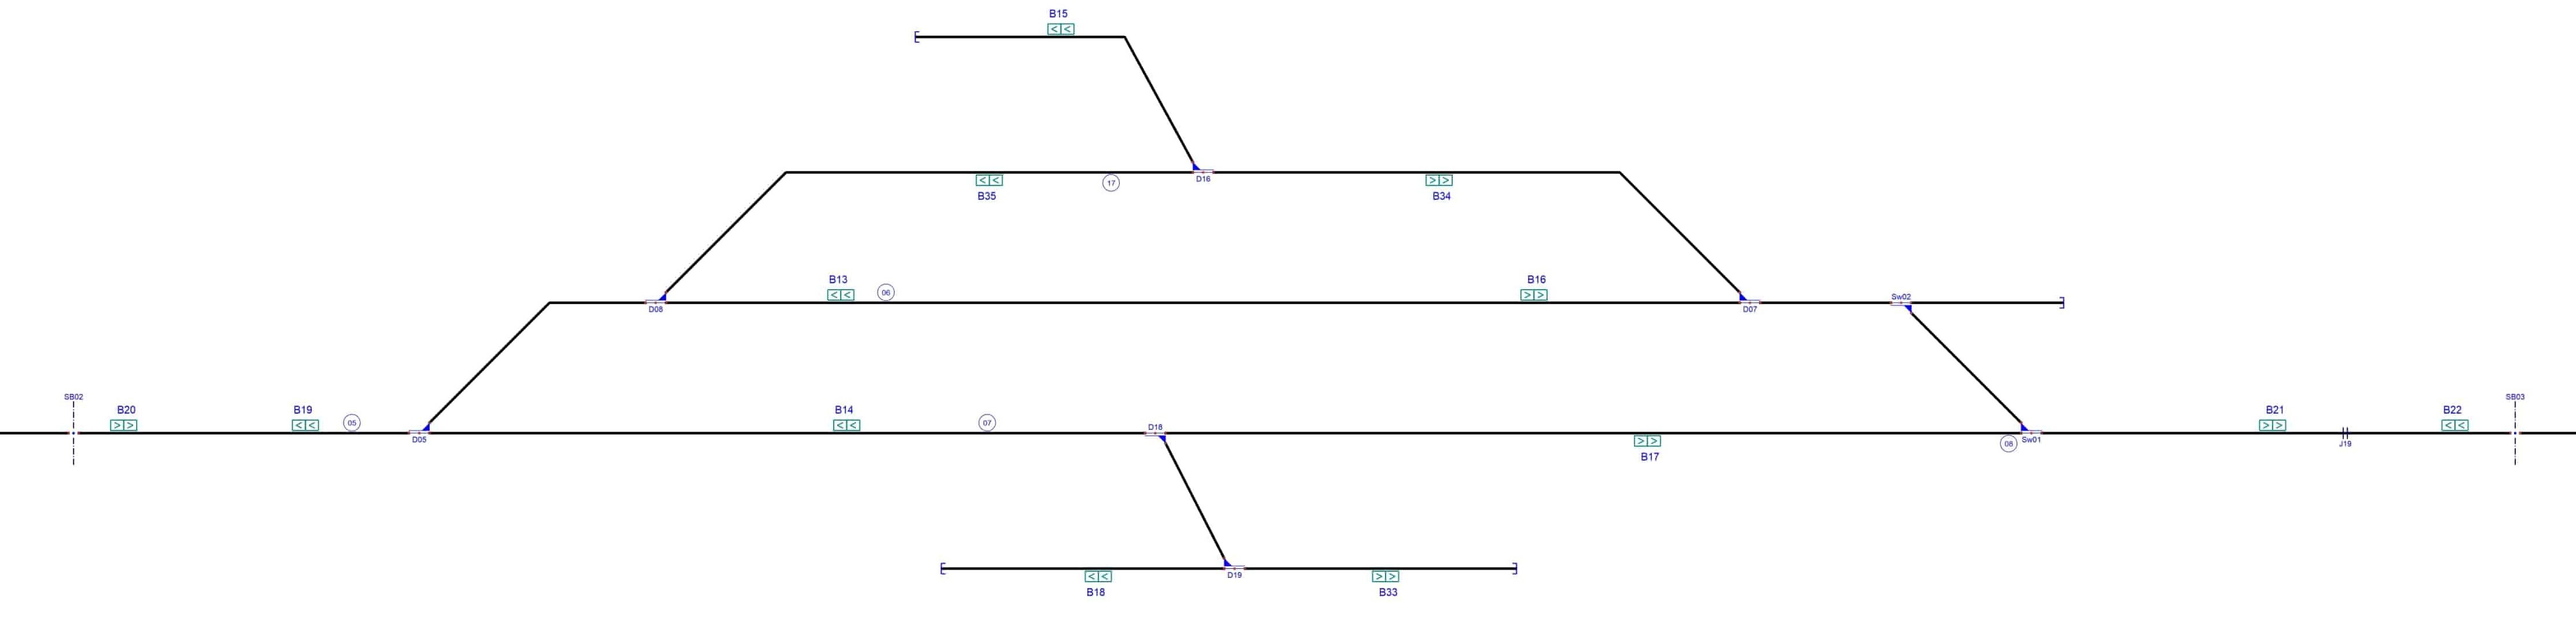
\includegraphics[width=1\textwidth]{resultados-obtenidos/ejemplo4/images/4_empty.png}
		\centering\caption{Topología ferroviaria del ejemplo 4 sin señalamiento.}
		\label{fig:EJ4_1}
	\end{figure}
	
	Esta topología tiene la particularidad de que las tres estaciones son prácticamente idéntica, salvo algunas variaciones. Por ejemplo, la tercer estación incluye un cambio de vías dobles como parte anidada de otros cambios de vías simples, lo cual no se había analizado en otros ejemplos. No obstante, se espera que el señalamiento sea similar en las tres estaciones.
